We propose a parallel algorithm based in the construct of the
\emph{Range Min-Max Tree}, {\tt
  RMMT}\cite{Navarro:2014:FFS:2620785.2601073}. Our algorithm, called
\emph{Parallel Succinct Tree Algorithm}, {\tt PSTA}, has as input a
possibly non-balanced parentheses sequence $P$, of moderate size
$|P|\leq N = w^{c}$, where $w$ is the length of the machine word and
$c\geq 1$ any constant.

The {\tt RMMT} is constructed over $P$, partitioning $P$ in disjoint
chunks of size $s$. Considering those chunks, the construction of the
{\tt RMMT} is based in the computation of different arrays of size
$O(\frac{|P|}{s})$. Such arrays are $e^{\prime}$, saving the final
excess of each chunk, $m^{\prime}$, saving the minimum excess value of
each chunk, $M^{\prime}$, saving the maximum excess value of each
chunk and $n^{\prime}$, saving the number of ocurrences of the minimum
value of each chunk. As a reminder, the excess value at position $i$
is:
\begin{equation}
  \displaystyle E[i] = \sum_{k=0}^{i} \pi(P[k])
  \label{eq:excess}
\end{equation}

where $\pi(``(") = 1$ and $\pi(``)") = -1$. See Figure
\ref{fig:RangeMinMaxTree} as an example of {\tt RMMT}, with $s=3$ and
$k=3$.

\begin{figure}[ht]
  \centering
  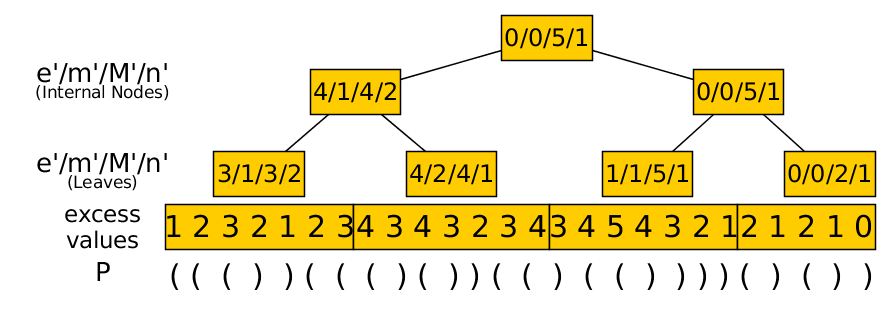
\includegraphics[scale=0.18]{./images/Range-min-max-tree.png}
  \caption{Range min-max tree}
  \label{fig:RangeMinMaxTree} 
\end{figure}

The first step of {\tt PSTA} is to compute the arrays $e^{\prime}$,
$m^{\prime}$, $M^{\prime}$ and $n^{\prime}$ in parallel. Since
$e^{\prime}$ just saves the last excess value of each chunk, which is
a sum, {\tt PSTA} needs to apply a parallel list-ranking
algorithm. Computing the last element of $e^{\prime}$, at position
$\frac{|P|}{s}-1$, we indirectly compute the rest of the elements of
$e^{\prime}$. We adapted the algorithm in \cite{Helman2001265} for
this context, computing $e^{\prime}$ in $O(\frac{|P|}{p})$ time, using
$p$ threads. Note that we do not need to compute more elements of
$e^{\prime}$ to the internal nodes of the {\tt RMMT}. The final size
of $e^{\prime}$ and the memory used in construction time are bounded
by $O(\frac{nc\lg(w)}{w})$ bits, where $c\geqslant 1$ and $w$ is the
word size in the RAM model.

To compute $m^{\prime}$, let's assume, without loss of generality,
that $p = k^{i}$, where $k = \Theta(\frac{w}{c\lg(w)})$ is the arity
of the internal nodes in the {\tt RMMT} and $i > 0$. {\tt PSTA}
assigns one thread per sub-tree of size $O(\frac{|P|}{sp})$, at level
$i$. So, it is possible to compute the $m^{\prime}$ values in all
sub-trees, in parallel, in $O(\frac{|P|}{sp}k)$ time. Then, for the
rest $O(p)$ nodes in the top of the tree, we compute the corresponding
minimum values in $O(k\lg_{k} p)$ time, computing each level in $O(k)$
time, just looking the $k$ values on the previous level using one
thread per vertex. If we consider $k$ as a constant, we can compute
$m^{\prime}$ in
$O(\frac{|P|}{sp}k + \lg p) = O(\frac{|P|}{p\lg(w)}+\lg p)$ time,
using $O(\frac{|P|c\lg(w)}{w})$ bits in construction time and in the
final array. Note that this solution makes sense considering that
$p\ll |P|$. Figure \ref{fig:min-max-array} illustrates the solution
explained here. We can compute $M^{\prime}$ and $n^{\prime}$ in the
same way, obtaining the same complexity.

\begin{figure}[ht]
  \centering
  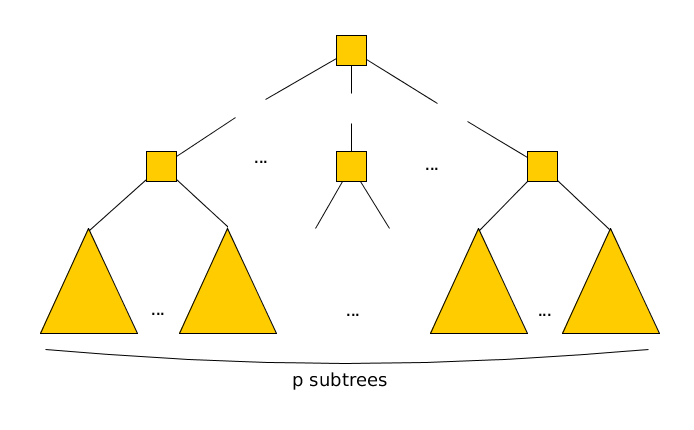
\includegraphics[scale=0.28]{./images/Min-Max-array.png}
  \caption{Computation of $m^{\prime}$ and $M^{\prime}$}
  \label{fig:min-max-array} 
\end{figure}

In addition to the arrays, the construction of the {\tt RMMT} involves
the computation of \emph{universal tables}. The universal tables are
used to support \emph{fwd\_search}($\bullet$),
\emph{bwd\_search}($\bullet$), \emph{rmqi}($\bullet$),
\emph{RMQi}($\bullet$), \emph{degree}($\bullet$) and
\emph{child}($\bullet$) queries in constant time. We can divide
universal tables into two types: those that depend on the leaves of
the {\tt RMMT} and those that depend on the internal nodes. In the
first case, we can compute each universal table in parallel assigning
one processor per leaf or chunk, which allows to compute different
parts of the table at the same time. For the second kind of tables, we
can assign one processor per internal node. Such processor computes
the section corresponding to that internal node in the universal
table. In that way, since computing the universal tables sequentially
has a complexity of $O(\sqrt{2^{w}}poly(w))$ time according to
\cite{Navarro:2014:FFS:2620785.2601073}, we can compute those
universal tables in $\displaystyle O(\frac{\sqrt{2^{w}}poly(w)}{p})$,
using $p$ processors.

To reduce the space used by the {\tt RMMT}, Sadakane and Navarro used
the results of \cite{Patrascu:2008:SUC:1470582.1470670}. They
represented the {\tt RMMT} as a \emph{aB-tree}, which is a complete
tree. As the {\tt RMMT} is also a complete, we can apply a
construction as that shown in Figure \ref{fig:min-max-array} to
construct the aB-tree. With respect to the universal tables needed in
the aB-tree, they can be computed following the same strategy
explained previously, but now with size $O(\sqrt{2^{w}})$
bits. Although we can apply a similar strategy, the results of
\cite{Patrascu:2008:SUC:1470582.1470670} are not practical, so we did
not implement this part of our solution. Available implementations of
the {\tt RMMT} do not implement this part either.

Finally, we can modify Theorem 4 of
\cite{Navarro:2014:FFS:2620785.2601073} as follows:
			
\newtheorem{theorem}{Threorem}
\begin{theorem}
  {\sc (modified from Thm. 4 in
    \cite{Navarro:2014:FFS:2620785.2601073})} On a $w$-bit word RAM,
  for any constant $c>\frac{3}{2}$, we can represent a sequence $P$ of
  $N=B^{c}$ parentheses, for sufficiently small
  $B=\Theta(\frac{w}{c\lg(w)})$, computing all operations of Table 1
  of \cite{Navarro:2014:FFS:2620785.2601073} in $O(c)$ time, with data
  structure depending on $P$ that uses $N+2$ bits, and universal
  tables (i.e., not depending on $P$) that use $O(\sqrt{2^{w}})$
  bits. The preprocessing time is $O(\frac{N}{p} + \log p)$, using $p$
  processors, and its working space is $O(N\log N)$ bits.
\end{theorem}
				
When we talk about a $w$-bit word RAM, we mean a model that supports
parallelism and can manipulate $w$ bits in $O(1)$. DYM meets these
criteria. Additionally, we consider that the overhead (in space and
time) imposed by the scheduling of processors is negligible. This is
reflected in the assumption $ N\gg p$ and in the results of
\cite{Blumofe:1999:SMC:324133.324234}.

As we mentioned above, the input to {\tt RMMT} consists of a
parentheses sequence $P$. However, sometimes $P$ is not available,
instead we have un ordinal tree, $T$. The construction of $P$ from $T$
has not been considered in previous implementations of the {\tt
  RMMT}. Here, we proposed an algorithm to compute $P$ in parallel,
complementing the {\tt PSTA} algorithm. We will call this algorithm
\emph{Parallel Folklore Enconding Algorithm}, {\tt PFEA}. The key
observation to obtain $P$ is that each parenthesis associated to an
edge $(u,v)$, ``('' or ``)'', is followed in the enconding by a
parenthesis associated to the edge $(parent(u), v)$, $(v, first(v))$
or $(u, next(u,v))$. All of them at distance of 1 of the edge
$(u,v)$. In the observation, $parent(u)$ is the parent node $u$,
$first(v)$ is the first child of $v$ and $next(u,v)$ is the child of
$u$ that succeeds the node $v$ in the array or children. With this
observation in mind, the core of {\tt PFEA} works as follows: Let
$(u,v)$ be an edge of $T$, where $u$ is parent of $v$ and let
$(u,v)_{0}$ ($(u,v)_{1}$) the opened (closed) parenthesis associated
to $(u,v)$. First, if $v$ is a leaf, then $(u,v)_{0}$ is followed by
$(u,v)_{1}$. If $v$ is not a leaf, then $(u,v)_{0}$ is followed by
$(v,first(v))_{0}$. If $v$ is not the last child of $u$,then
$(u,v)_{1}$ is followed by $(u,next(u,v))_{0}$. Finally, if $v$ is the
last child of $u$, then $(u,v)_{1}$ is followed by
$(u,parent(u))_{1}$. In the next section we will give more details of
{\tt PFEA} algorithm.
